\documentclass[11pt,a4paper,fontset=fandol]{ctexart}

\usepackage[a4paper,margin=2.2cm]{geometry}
\usepackage{graphicx}
\usepackage{float}
\usepackage{booktabs}
\usepackage{longtable}
\usepackage{array}
\usepackage{xcolor}
\usepackage{hyperref}
\usepackage{tikz}
\usepackage{enumitem}
\usepackage{listings}
\usetikzlibrary{arrows.meta,positioning,shapes.geometric,fit,calc}

\definecolor{ink}{HTML}{25313B}
\definecolor{muted}{HTML}{64748B}
\definecolor{blue}{HTML}{2563EB}
\definecolor{green}{HTML}{059669}
\definecolor{orange}{HTML}{D97706}
\definecolor{red}{HTML}{DC2626}
\definecolor{paper}{HTML}{F8FAFC}
\definecolor{line}{HTML}{CBD5E1}

\hypersetup{
  colorlinks=true,
  linkcolor=blue,
  urlcolor=blue,
  citecolor=green
}

\lstdefinestyle{code}{
  basicstyle=\ttfamily\small,
  breaklines=true,
  columns=fullflexible,
  frame=single,
  rulecolor=\color{line},
  backgroundcolor=\color{paper},
  xleftmargin=0.5em,
  xrightmargin=0.5em
}
\lstset{style=code}

\newcommand{\code}[1]{\texttt{#1}}
\newcommand{\repoPath}[1]{\texttt{#1}}

\title{\textbf{EventStoryLine 项目结构学习说明}\\
\large 面向 VS Code 阅读与二次开发的导览}
\author{yifeng\_study}
\date{2026 年 5 月 7 日}

\begin{document}
\maketitle

\begin{figure}[H]
  \centering
  
\includegraphics[width=0.95\linewidth]{assets/cover_learning.png}
  \caption{学习这个仓库时，可以把它想成“语料数据 + 转换脚本 + 基线系统 + 评测”的组合。}
\end{figure}

\tableofcontents
\newpage

\section{一句话理解这个项目}

\textbf{EventStoryLine} 仓库围绕 ESC（事件故事线语料库）和 ECB+ 语料展开，核心目标是支持新闻事件故事线中的事件关系抽取、数据格式转换、基线系统运行与结果评测。

从当前项目结构看，它不是一个典型 Web/App 工程，而更像一个\textbf{研究型 NLP 语料仓库}：

\begin{itemize}[leftmargin=2em]
  \item 大量 XML/NAF/评测格式文件保存语料和标注。
  \item 少量 Python 脚本负责把 CAT XML 标注转换成评测格式。
  \item 基线脚本基于事件共现、PPMI、时间锚等启发式方法生成系统输出。
  \item 评测脚本比较标准答案文件与基线输出，计算精确率、召回率、F1。
\end{itemize}

\section{项目顶层目录}

当前仓库顶层最重要的内容如下：

\begin{longtable}{>{\ttfamily}p{0.31\linewidth}p{0.61\linewidth}}
\toprule
\normalfont 路径 & 作用 \\
\midrule
README.md & 项目说明、版本信息和引用论文。 \\
LICENSE.md & 许可证文件。 \\
ECB+\_LREC2014/ & 原始 ECB+ 相关材料，包括 ECB+ XML、README、license 和压缩包。 \\
annotated\_data/ & ESC 的 CAT/XML 标注数据，按版本和 topic 组织。 \\
evaluation\_format/ & 已转换好的评测格式数据，分全语料和测试语料。 \\
ecb+\_naf/ & ECB+ 的 NAF 版本文件，基线脚本中用于读取 lemma、句子等语言学信息。 \\
ppmi\_events\_ecb+\_test/ & PPMI 基线相关的事件数据或中间测试材料。 \\
create\_gold\_document.py & 从 ECB+ 与 ESC CAT XML 合并生成评测格式标准答案文件。 \\
baseline\_OP.py & 简单共现基线：同一句事件两两成对。 \\
baseline\_PPMI1.py & 使用 PPMI 的故事线基线。 \\
baseline\_PPMI\_CONTAINS.py & 在 PPMI 基础上加入时间锚 CONTAINS 限制的基线。 \\
eval\_script.py & 对系统输出和标准答案进行精确率、召回率、F1 评测。 \\
yifeng\_study/ & 本学习文档所在目录。 \\
\bottomrule
\end{longtable}

\begin{figure}[H]
\centering
\begin{tikzpicture}[
  font=\small,
  node distance=5mm,
  folder/.style={draw=line, fill=paper, rounded corners=2pt, inner xsep=7pt, inner ysep=4pt, align=left},
  root/.style={draw=blue, fill=blue!8, rounded corners=2pt, inner xsep=8pt, inner ysep=5pt, font=\bfseries}
]
\node[root] (root) {EventStoryLine/};
\node[folder, below left=8mm and 15mm of root] (data) {数据目录\\
\code{ECB+\_LREC2014}\\
\code{annotated\_data}\\
\code{evaluation\_format}\\
\code{ecb+\_naf}};
\node[folder, below=8mm of root] (scripts) {Python 脚本\\
\code{create\_gold\_document.py}\\
\code{baseline\_*.py}\\
\code{eval\_script.py}};
\node[folder, below right=8mm and 15mm of root] (study) {学习区\\
\code{yifeng\_study}\\
\code{assets}\\
\code{project\_structure\_guide.tex}};
\draw[-{Stealth[length=2mm]}, blue] (root) -- (data);
\draw[-{Stealth[length=2mm]}, blue] (root) -- (scripts);
\draw[-{Stealth[length=2mm]}, blue] (root) -- (study);
\end{tikzpicture}
\caption{顶层结构可以粗略分为数据、脚本、学习文档三块。}
\end{figure}

\section{数据目录怎么读}

\subsection{\code{annotated\_data/}：ESC 的 CAT/XML 标注}

这个目录保存 ESC 的人工/众包故事线标注，当前有多个版本：

\begin{itemize}[leftmargin=2em]
  \item \code{v0.9}：早期版本。
  \item \code{v1.0}：专家标注版本。
  \item \code{v1.5}：专家 + 众包扩展版本，README 中说明了 \code{origin} 和 \code{validated} 等属性。
\end{itemize}

其下再按 topic 编号划分，例如：

\begin{lstlisting}
annotated_data/v1.5/22/22_3ecbplus.xml.xml
annotated_data/v1.5/14/14_11ecbplus.xml.xml
\end{lstlisting}

注意文件名里常见 \code{.xml.xml}，这是仓库已有数据命名，不是 LaTeX 或 VS Code 的问题。

\subsection{\code{ECB+\_LREC2014/}：ECB+ 原始语料}

\code{create\_gold\_document.py} 会同时读取：

\begin{itemize}[leftmargin=2em]
  \item ECB+ 原始 CAT 文件，用于事件提及和共指链；
  \item ESC 标注文件，用于 PLOT\_LINK 关系；
  \item 然后把共指扩展后的事件关系写到评测格式文件。
\end{itemize}

\subsection{\code{evaluation\_format/}：模型和评测最常用的格式}

这个目录已经把 XML 标注转换成更容易评测的 TSV 风格文本行。主要分两大块：

\begin{itemize}[leftmargin=2em]
  \item \code{full\_corpus/}：全语料评测格式。
  \item \code{test\_corpus/}：测试集评测格式。
\end{itemize}

每个版本下面常见两个子目录：

\begin{itemize}[leftmargin=2em]
  \item \code{coref\_chain/}：共指链扩展后的事件链关系。
  \item \code{event\_mentions\_extended/}：扩展到事件提及对级别的事件关系。
\end{itemize}

评测格式的一行一般类似：

\begin{lstlisting}
event_token_ids_source    event_token_ids_target    RELATION_TYPE
\end{lstlisting}

\section{核心概念图}

\begin{figure}[H]
  \centering
  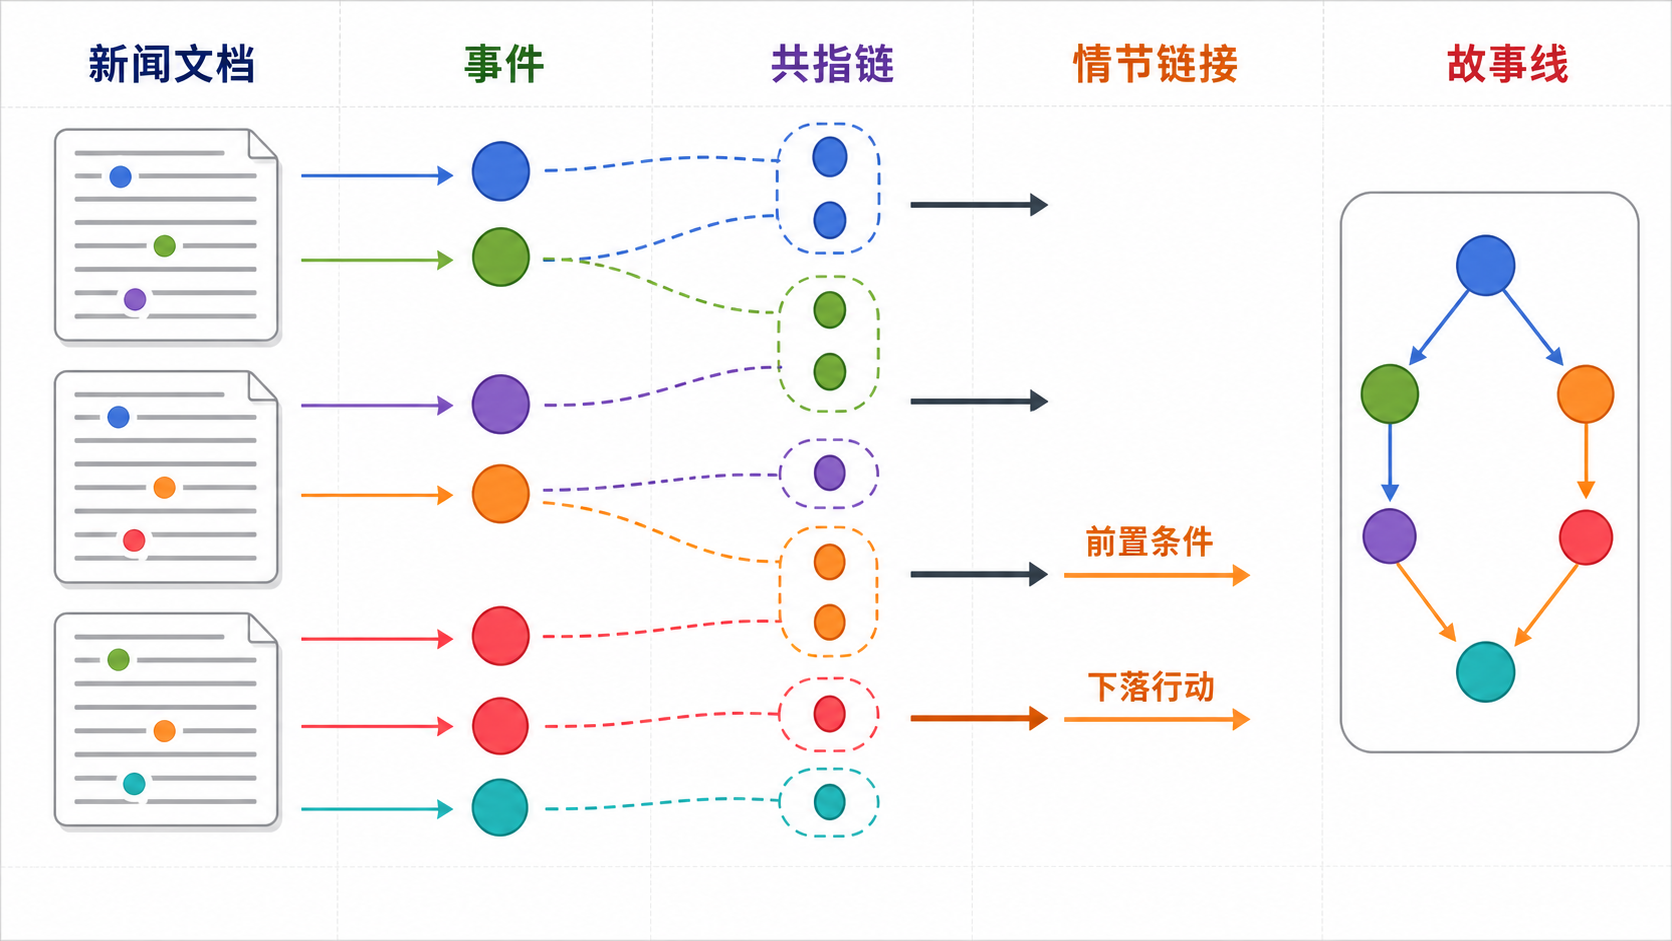
\includegraphics[width=0.95\linewidth]{assets/storyline_concept.png}
  \caption{文档、事件提及、共指、情节链接和故事线之间的直观关系。}
\end{figure}

\begin{figure}[H]
\centering
\begin{tikzpicture}[
  font=\small,
  box/.style={draw=line, fill=paper, rounded corners=2pt, minimum width=28mm, minimum height=9mm, align=center},
  rel/.style={-{Stealth[length=2mm]}, thick},
  note/.style={draw=line, fill=orange!8, rounded corners=2pt, align=center, inner sep=5pt}
]
\node[box] (doc) {新闻文档};
\node[box, right=14mm of doc] (mention) {事件提及};
\node[box, right=14mm of mention] (coref) {共指关系\\事件链};
\node[box, below=13mm of coref] (plot) {PLOT\_LINK\\事件关系};
\node[box, left=14mm of plot] (story) {Storyline\\故事线};
\node[note, below=11mm of mention] (rels) {常见关系标签\\PRECONDITION\\FALLING\_ACTION};

\draw[rel, blue] (doc) -- (mention);
\draw[rel, green] (mention) -- (coref);
\draw[rel, orange] (coref) -- (plot);
\draw[rel, red] (plot) -- (story);
\draw[rel, orange!80!black] (rels) -- (plot);
\end{tikzpicture}
\caption{这个项目关心的不是普通实体分类，而是事件之间如何组成故事线。}
\end{figure}

\section{脚本职责}

\subsection{\code{create\_gold\_document.py}}

这个脚本是理解数据流的入口。它把 ECB+ 与 ESC 两边的信息合并，生成评测用标准答案文件。

主要函数：

\begin{longtable}{>{\ttfamily}p{0.34\linewidth}p{0.58\linewidth}}
\toprule
\normalfont 函数 & 作用 \\
\midrule
extract\_event\_CAT & 从 CAT XML 的 Markables 中抽取 ACTION / NEG\_ACTION 类事件。 \\
extract\_corefRelations & 从 ECB+ Relations 中抽取事件共指链。 \\
extract\_plotLink & 从 ESC XML 中抽取 PLOT\_LINK 关系及其 relType。 \\
create\_merged\_files & 把共指扩展应用到情节链接，写出两个评测文件。 \\
merge\_annotations & 遍历 topic 文件夹，批量调用合并逻辑。 \\
\bottomrule
\end{longtable}

运行方式：

\begin{lstlisting}[language=bash]
python3 create_gold_document.py ECBplusTopic ECBstarTopic outfolder
\end{lstlisting}

\subsection{\code{baseline\_OP.py}}

这是最容易读懂的基线脚本。它假设：

\begin{itemize}[leftmargin=2em]
  \item 事件已经被正确识别；
  \item 同一句子中的事件两两之间都有 PLOT\_LINK；
  \item 过滤掉 reporting、causative、aspectual 等不适合的事件类别；
  \item 输出关系默认写成 \code{PRECONDITION}。
\end{itemize}

它适合当作你阅读代码的第一站，因为逻辑从 XML 解析到事件配对非常直接。

\subsection{\code{baseline\_PPMI1.py}}

这个基线更像研究实验脚本。它读取 CAT 与 NAF：

\begin{itemize}[leftmargin=2em]
  \item CAT 提供事件提及和 token id。
  \item NAF 提供 lemma、句子编号等语言学信息。
  \item 使用事件 lemma 的共现统计计算 PPMI。
  \item 用 PPMI 阈值筛选候选事件对。
\end{itemize}

\subsection{\code{baseline\_PPMI\_CONTAINS.py}}

这个脚本继承 PPMI 思路，但额外利用 TLINK 中的 \code{CONTAINS} 时间锚关系。它的直觉是：如果事件共享某个时间锚，可能更值得考虑为故事线关系候选。

\subsection{\code{eval\_script.py}}

评测脚本读取标准答案与系统输出，计算两种层面的指标：

\begin{itemize}[leftmargin=2em]
  \item \textbf{事件对层面}：只看事件对是否匹配。
  \item \textbf{事件对 + 关系类型层面}：事件对和关系类型都要匹配。
\end{itemize}

运行方式：

\begin{lstlisting}[language=bash]
python3 eval_script.py gold_dir system_dir
\end{lstlisting}

\section{数据处理流程}

\begin{figure}[H]
  \centering
  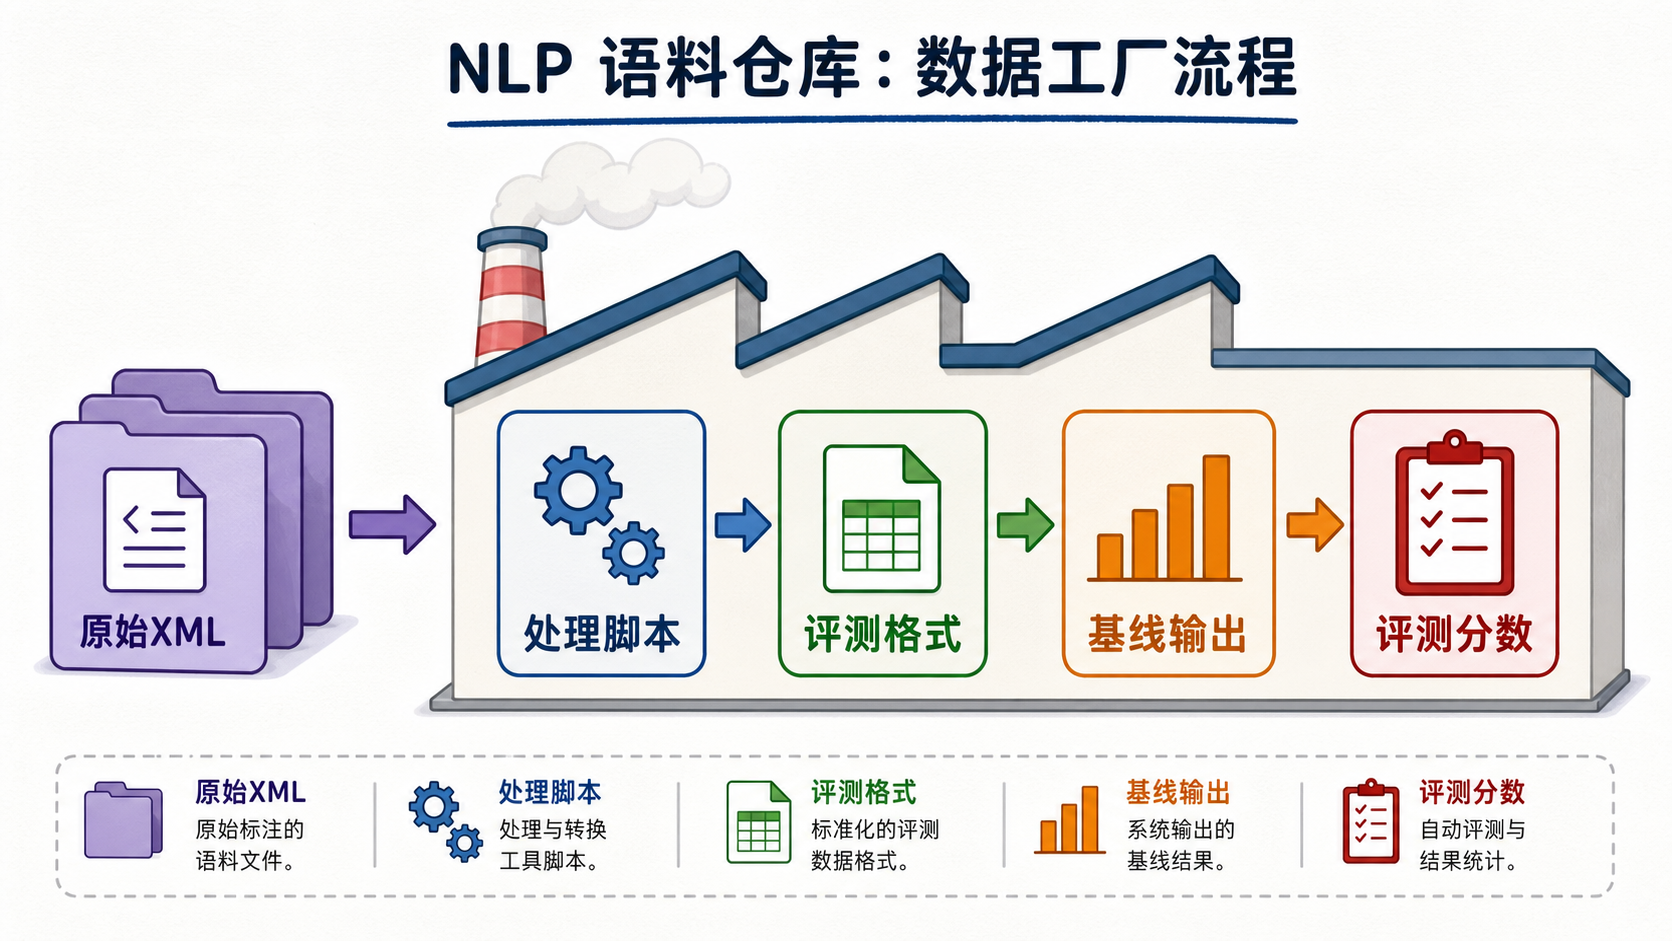
\includegraphics[width=0.95\linewidth]{assets/data_factory.png}
\caption{仓库的数据处理可以看成从 XML 标注到评测格式，再到基线输出和分数。}
\end{figure}

\begin{figure}[H]
\centering
\begin{tikzpicture}[
  font=\small,
  step/.style={draw=line, fill=paper, rounded corners=2pt, minimum width=34mm, minimum height=10mm, align=center},
  data/.style={draw=blue!50, fill=blue!7, rounded corners=2pt, minimum width=35mm, minimum height=10mm, align=center},
  script/.style={draw=green!50!black, fill=green!8, rounded corners=2pt, minimum width=35mm, minimum height=10mm, align=center},
  outputbox/.style={draw=orange!70!black, fill=orange!10, rounded corners=2pt, minimum width=35mm, minimum height=10mm, align=center},
  arr/.style={-{Stealth[length=2mm]}, thick}
]
\node[data] (ecb) {ECB+ CAT XML\\事件 + coref};
\node[data, below=8mm of ecb] (esc) {ESC CAT XML\\PLOT\_LINK};
\node[script, right=19mm of $(ecb)!0.5!(esc)$] (gold) {\code{create\_gold}\\合并标注};
\node[outputbox, right=19mm of gold] (eval) {评测\\格式};
\node[script, below=12mm of eval] (base) {基线\\脚本};
\node[outputbox, left=19mm of base] (sys) {系统\\输出};
\node[script, left=19mm of sys] (score) {\code{eval\_script}\\P/R/F1};

\draw[arr, blue] (ecb) -- (gold);
\draw[arr, blue] (esc) -- (gold);
\draw[arr, green!50!black] (gold) -- (eval);
\draw[arr, orange!80!black] (eval) -- (base);
\draw[arr, orange!80!black] (base) -- (sys);
\draw[arr, red] (sys) -- (score);
\draw[arr, red] (eval.south west) to[out=210,in=50] (score.north east);
\end{tikzpicture}
\caption{推荐按这条路径理解代码：先看标准答案如何生成，再看基线如何输出，最后看评测如何计分。}
\end{figure}

\section{当前仓库的数量感}

下面是写文档时对当前工作区做的粗略文件计数，帮助你判断哪里是大头：

\begin{center}
\begin{tabular}{lrr}
\toprule
目录 & 文件数 & 阅读优先级 \\
\midrule
\code{annotated\_data/} & 1103 & 中：了解数据结构即可，不必逐个读。 \\
\code{ECB+\_LREC2014/} & 990 & 中：原始语料，主要配合脚本理解。 \\
\code{evaluation\_format/} & 2602 & 高：评测输入和输出最常用。 \\
\code{ecb+\_naf/} & 272 & 中：PPMI 基线需要。 \\
\code{ppmi\_events\_ecb+\_test/} & 224 & 低到中：基线相关材料。 \\
\bottomrule
\end{tabular}
\end{center}

\section{推荐学习路线}

\begin{enumerate}[leftmargin=2em]
  \item 先读 \code{README.md}，弄清楚 ESC v1.0、v1.2、v1.5 的差异。
  \item 打开 \code{evaluation\_format/test\_corpus/v1.5/event\_mentions\_extended/} 里的任意文件，看三列格式。
  \item 读 \code{eval\_script.py}，因为它最短，能快速说明系统输出应该长什么样。
  \item 读 \code{baseline\_OP.py}，理解“同句事件两两配对”的最朴素基线。
  \item 再读 \code{create\_gold\_document.py}，理解 XML 标注如何变成评测格式。
  \item 最后读 \code{baseline\_PPMI1.py} 和 \code{baseline\_PPMI\_CONTAINS.py}，它们更偏实验细节。
\end{enumerate}

\section{VS Code 里怎么打开}

建议在 VS Code 中打开整个仓库目录：

\begin{lstlisting}[language=bash]
code /Users/luyifeng/Documents/GitHub/EventStoryLine
\end{lstlisting}

然后重点看：

\begin{lstlisting}
yifeng_study/project_structure_guide.tex
yifeng_study/assets/
README.md
eval_script.py
baseline_OP.py
create_gold_document.py
\end{lstlisting}

如果安装了 LaTeX Workshop 插件，可以用 XeLaTeX 编译本文档。中文文档建议使用 \code{xelatex}，不要用普通 \code{pdflatex}。

\section{速查：脚本输入输出}

\begin{longtable}{>{\ttfamily}p{0.24\linewidth}p{0.29\linewidth}p{0.35\linewidth}}
\toprule
\normalfont 脚本 & 输入 & 输出/作用 \\
\midrule
create\_gold\_document.py & ECB+ 主题目录、ESC 主题目录、输出目录 & 标准答案评测格式文件。 \\
baseline\_OP.py & ECB+ 主题目录、输出目录 & \code{*.base.out} 系统输出。 \\
baseline\_PPMI1.py & CAT/NAF/PPMI 相关输入 & PPMI 筛选后的事件关系输出。 \\
baseline\_PPMI\_CONTAINS.py & CAT/NAF/时间锚相关输入 & 加入 CONTAINS 限制的 PPMI 输出。 \\
eval\_script.py & 标准答案目录、系统输出目录 & 事件对层面与关系类型层面的精确率、召回率、F1。 \\
\bottomrule
\end{longtable}

\section{读代码时的几个提醒}

\begin{itemize}[leftmargin=2em]
  \item 这个仓库代码年份较早，有些 lxml API 如 \code{getchildren()} 在新版本里可能会有兼容性提醒。
  \item 脚本大量使用追加写入 \code{"a"}，重复运行同一个输出路径可能导致结果叠加；学习时最好输出到新的临时目录。
  \item 文件名包含 \code{+}、下划线和双扩展名，命令行里路径要小心复制完整。
  \item 基线不是深度学习模型，而是用于论文实验的启发式系统。
\end{itemize}

\end{document}
